\documentclass[12pt]{article}
\usepackage{amsmath, amssymb}
\usepackage{hyperref}
\usepackage{graphicx}
\usepackage{tikz}
\setlength{\parindent}{0pt}

\title{Probearbeit 1}
\author{}
\date{03.12.2025}

\begin{document}
\maketitle

\textbf{Hinweis.} Begründe alle Schritte. Exakte Werte sind ausreichend. Skizzen müssen nicht maßstäblich sein, aber wichtige Punkte sollen beschriftet werden.

\section*{Aufgabe 1: Scheitelpunkt ablesen}
Betrachte \(f(x) = (x-1)^{2} - 4\).
\begin{enumerate}
  \item Berechne \(f(x)\) für \(x = -1, 0, 1, 2, 3\) und trage die Werte in die Tabelle ein.
  \item Gib Scheitelpunkt, Symmetrieachse und Öffnungsrichtung der Parabel an.
  \item Zeichne die Parabel mithilfe der berechneten Punkte. Trage Scheitelpunkt und Symmetrieachse im Koordinatensystem unten ein.
\end{enumerate}

\begin{center}
\begingroup
\renewcommand{\arraystretch}{1.8}
\begin{tabular}{|c|c|c|c|c|c|}
  \hline
  \(x\) & \(-1\) & \(0\) & \(1\) & \(2\) & \(3\) \\
  \hline
  \(y = f(x)\) & & & & & \\
  \hline
\end{tabular}
\endgroup
\end{center}

\begin{center}
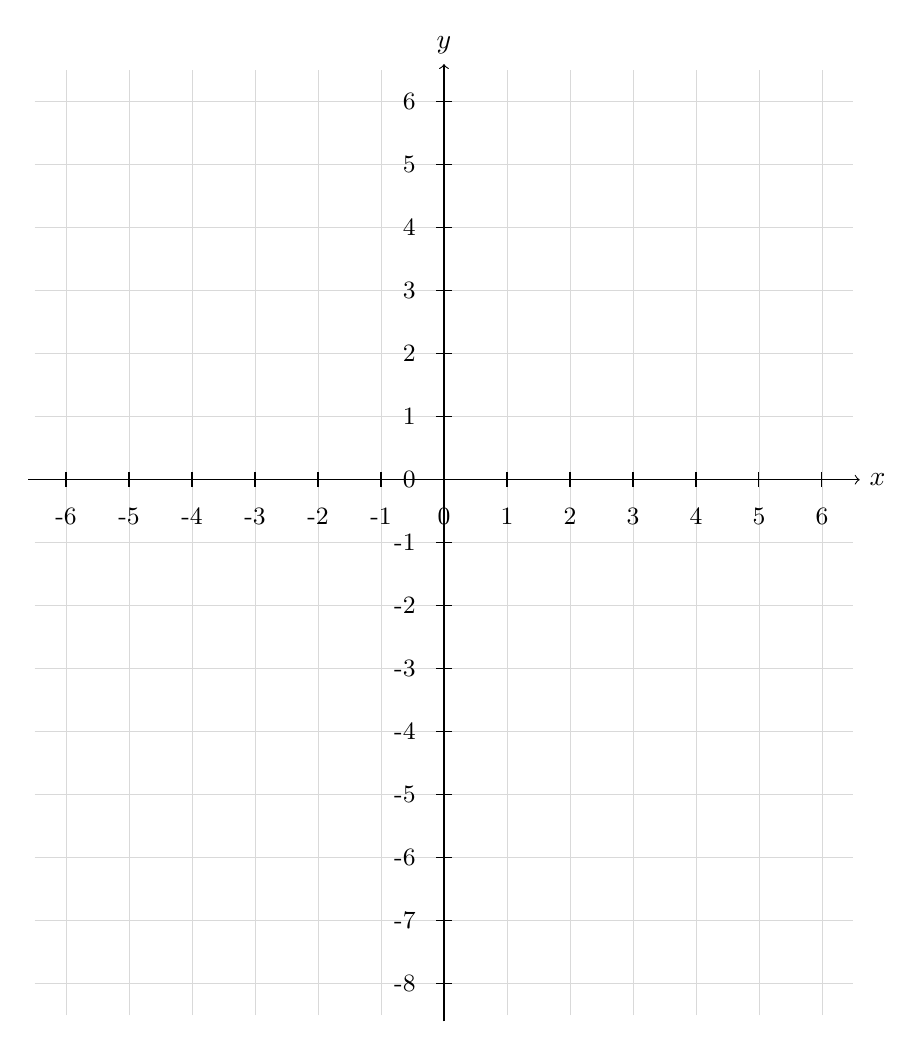
\begin{tikzpicture}[scale=0.8]
  \draw[step=1cm,gray!30,very thin] (-6.5,-8.5) grid (6.5,6.5);
  \draw[->] (-6.6,0) -- (6.6,0) node[right] {$x$};
  \draw[->] (0,-8.6) -- (0,6.6) node[above] {$y$};
  \foreach \x in {-6,-5,...,6} \draw (\x,0.12) -- (\x,-0.12) node[below=4pt] {\small \x};
  \foreach \y in {-8,-7,...,6} \draw (0.12,\y) -- (-0.12,\y) node[left=4pt] {\small \y};
\end{tikzpicture}
\end{center}

\section*{Aufgabe 2: Nullstellen mit der PQ-Formel}
Die PQ-Formel für \(x^{2} + px + q = 0\) lautet
\[
  x_{1,2} = -\frac{p}{2} \pm \sqrt{\left(\frac{p}{2}\right)^{2} - q}.
\]
Verwende sie, um die \(x\)-Achsenabschnitte von \(y = x^{2} - 6x + 5\) zu berechnen. Nenne beide Nullstellen und gib an, ob die Parabel die \(x\)-Achse dort schneidet oder berührt.

\section*{Aufgabe 3: Skizze aus der Funktionsgleichung}
Skizziere den Graphen von \(g(x) = -\tfrac{1}{2}(x-3)^{2} + 4\) im Koordinatensystem. Beschrifte Scheitelpunkt, \(y\)-Achsenabschnitt und vorhandene \(x\)-Achsenabschnitte.

\begin{center}
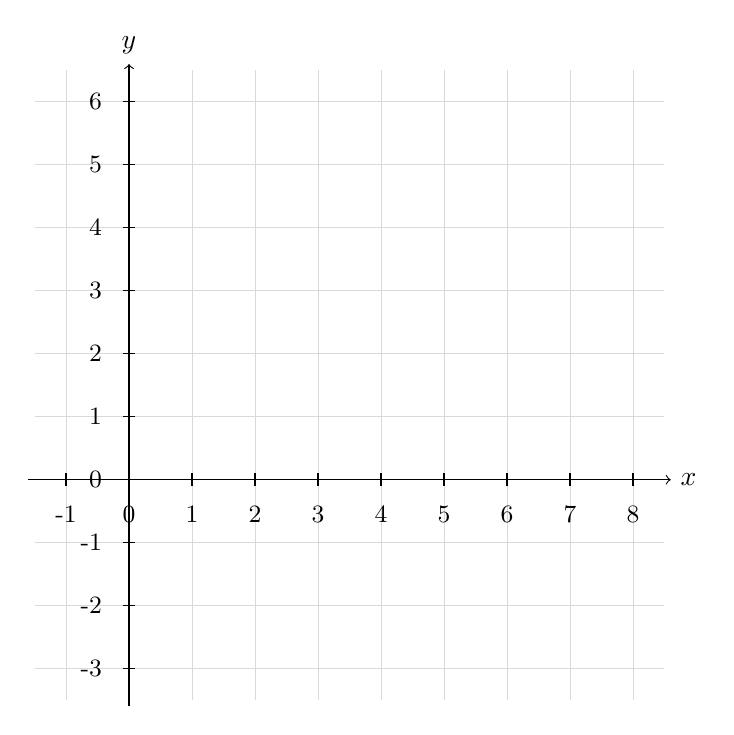
\begin{tikzpicture}[scale=0.8]
  \draw[step=1cm,gray!30,very thin] (-1.5,-3.5) grid (8.5,6.5);
  \draw[->] (-1.6,0) -- (8.6,0) node[right] {$x$};
  \draw[->] (0,-3.6) -- (0,6.6) node[above] {$y$};
  \foreach \x in {-1,0,...,8} \draw (\x,0.1) -- (\x,-0.1) node[below=4pt] {\small \x};
  \foreach \y in {-3,-2,...,6} \draw (0.1,\y) -- (-0.1,\y) node[left=4pt] {\small \y};
\end{tikzpicture}
\end{center}

\section*{Aufgabe 4: Tiefpunkt einer nach oben offenen Parabel}
Für \(h(x) = 2x^{2} - 8x + 1\):
\begin{enumerate}
  \item Schreibe \(h(x)\) in Scheitelpunktform und bestimme die Koordinaten des Tiefpunkts.
  \item Gib den minimalen Funktionswert und die Gleichung der Symmetrieachse an.
\end{enumerate}

\end{document}
